\chapter{Aggregate Supply and Aggregate Demand (Text Ch. 26)}

The AS--AD model explains how real GDP and the price level are determined and how they
interact. It is the main framework for understanding the business cycle, inflation and
the effects of fiscal and monetary policy.

\section{Aggregate supply}

\subsection{Quantity supplied and supply}

The \emph{quantity of real GDP supplied} ($Y$) is the total quantity of goods and
services, valued in constant base-year dollars, that firms plan to produce during a
given period. It depends on
\begin{itemize}
  \item the quantity of labour employed,
  \item the quantities of physical and human capital, and
  \item the state of technology.
\end{itemize}
At any given time, the quantity of capital and the state of technology are fixed; only the
quantity of labour can vary. The quantity of labour employed depends on decisions in the
labour market, so real GDP supplied varies with the labour market outcome.

\begin{definition}[Potential GDP]
\emph{Potential GDP} is the quantity of real GDP supplied at full employment (when the
unemployment rate equals the natural rate).
\end{definition}

\begin{definition}[Aggregate supply]
\emph{Aggregate supply} is the relationship between the quantity of real GDP supplied and
the price level. We distinguish the long run and the short run.
\end{definition}

\subsection{Long-run aggregate supply}

\begin{definition}[LRAS]
\emph{Long-run aggregate supply} is the relationship between the quantity of real GDP
supplied and the price level when real GDP equals potential GDP. The LRAS curve is
\emph{vertical} at potential GDP.
\end{definition}

Along the LRAS curve, when the price level rises, the money wage rate and other resource
prices rise by the same percentage. Relative prices, real wages and profits are unchanged,
so firms have no reason to change output, and real GDP stays at potential.

\subsection{Short-run aggregate supply}

\begin{definition}[SRAS]
\emph{Short-run aggregate supply} is the relationship between the quantity of real GDP
supplied and the price level when the money wage rate, the prices of other resources and
potential GDP remain constant. The SRAS curve slopes \emph{upward}.
\end{definition}

Why upward? With the money wage rate fixed, a rise in the price level lowers the real
wage, so firms' profits per unit rise and they hire more labour and produce more. A fall in
the price level raises the real wage, and firms cut output. The SRAS curve crosses LRAS at
the price level at which the money wage rate is consistent with full employment.

\subsection{Movements along and changes in aggregate supply}

A change in the price level causes a movement along the SRAS curve (and along LRAS, at
potential GDP). Aggregate supply \emph{changes} when an influence on production plans
other than the price level changes:
\begin{enumerate}
  \item \textbf{Changes in potential GDP} shift \emph{both} LRAS and SRAS by the same
        amount. Potential GDP increases if
        \begin{enumerate}
          \item the full-employment quantity of labour increases (population growth,
                immigration);
          \item the quantity of capital (physical or human) increases; or
          \item technology advances.
        \end{enumerate}
  \item \textbf{Changes in the money wage rate} (and other resource prices, e.g.\ the
        price of oil) shift \emph{only} SRAS. A rise in the money wage rate increases
        firms' costs and shifts SRAS leftward; LRAS does not move, because potential GDP
        does not depend on the money wage.
\end{enumerate}
The money wage rate changes because of a departure from full employment (unemployment
above the natural rate pushes it down; below pushes it up) and because of expected
inflation (workers bargain for higher money wages to protect their real wages).

\begin{center}
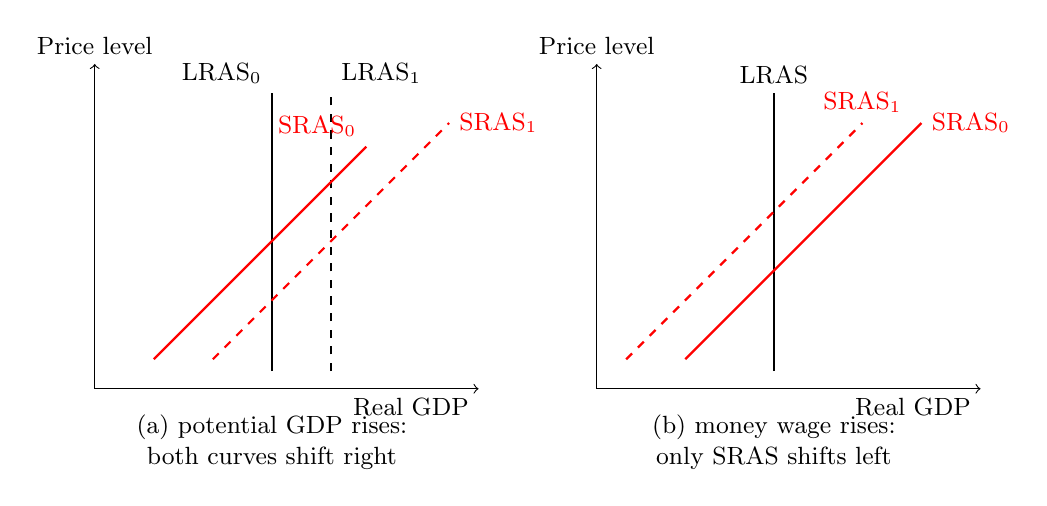
\begin{tikzpicture}[scale=0.75, every node/.style={font=\small}]
  \draw[->] (0,0) -- (6.5,0) node[below left] {Real GDP};
  \draw[->] (0,0) -- (0,5.5) node[above] {Price level};
  \draw[thick] (3,0.3) -- (3,5) node[above left] {LRAS$_0$};
  \draw[thick, dashed] (4,0.3) -- (4,5) node[above right] {LRAS$_1$};
  \draw[thick, red] (1,0.5) -- (4.6,4.1) node[above left] {SRAS$_0$};
  \draw[thick, red, dashed] (2,0.5) -- (6,4.5) node[right] {SRAS$_1$};
  \node[align=center] at (3,-0.9) {(a) potential GDP rises:\\both curves shift right};
  \begin{scope}[xshift=8.5cm]
    \draw[->] (0,0) -- (6.5,0) node[below left] {Real GDP};
    \draw[->] (0,0) -- (0,5.5) node[above] {Price level};
    \draw[thick] (3,0.3) -- (3,5) node[above] {LRAS};
    \draw[thick, red] (1.5,0.5) -- (5.5,4.5) node[right] {SRAS$_0$};
    \draw[thick, red, dashed] (0.5,0.5) -- (4.5,4.5) node[above] {SRAS$_1$};
    \node[align=center] at (3,-0.9) {(b) money wage rises:\\only SRAS shifts left};
  \end{scope}
\end{tikzpicture}
\end{center}

\section{Aggregate demand}

The \emph{quantity of real GDP demanded} is the total amount of final goods and services
produced in Canada that people, businesses, governments and foreigners plan to buy:
\[
  Y = C + I + G + (X - M).
\]

\begin{definition}[Aggregate demand]
\emph{Aggregate demand} is the relationship between the quantity of real GDP demanded and
the price level, other things remaining the same. The AD curve slopes \emph{downward}.
\end{definition}

Buying plans depend on many factors; the main ones are the price level, expectations,
fiscal and monetary policy, and the world economy.

\subsection{Why the AD curve slopes downward}

\begin{enumerate}
  \item \textbf{Wealth effect}: a rise in the price level, other things remaining the
        same, decreases the quantity of \emph{real} wealth (the real value of money,
        bonds and other assets). To restore their wealth, people save more and spend
        less, so the quantity of real GDP demanded decreases.
  \item \textbf{Substitution effects}:
        \begin{enumerate}
          \item \emph{Intertemporal substitution effect}: a rise in the price level, other
                things remaining the same, decreases the real value of money and raises
                the interest rate. Faced with a higher interest rate, people borrow and
                spend less now (substituting future for present spending).
          \item \emph{International substitution effect}: a rise in the Canadian price
                level, other things remaining the same, increases the price of
                Canadian-produced goods relative to foreign goods. Canadians buy more
                imports and foreigners buy fewer Canadian exports, so net exports fall.
        \end{enumerate}
\end{enumerate}

\begin{important}[Pitfall]
The AD curve is \emph{not} a market demand curve: it does not slope down because people
substitute toward cheaper goods within the economy. All Canadian prices rise together
along the AD curve; the slope comes from the three effects above.
\end{important}

\subsection{Changes in aggregate demand}

A change in any influence on buying plans other than the price level shifts the AD curve.
\begin{enumerate}
  \item \textbf{Expectations}: higher expected future income, higher expected inflation
        or higher expected future profits increase consumption and investment today, so AD
        increases (shifts rightward).
  \item \textbf{Fiscal policy and monetary policy}:
        \begin{enumerate}
          \item \emph{Fiscal policy} is the government's attempt to influence the economy
                by setting and changing taxes, making transfer payments and purchasing
                goods and services. A tax cut or an increase in transfers raises
                disposable income; an increase in government expenditure adds directly to
                AD. Both increase AD.
          \item \emph{Monetary policy} consists of changes in interest rates and in the
                quantity of money. A lower interest rate or more money increases AD.
        \end{enumerate}
  \item \textbf{The world economy}, in two ways:
        \begin{enumerate}
          \item a fall in the foreign exchange rate (depreciation of the Canadian dollar)
                lowers the price of Canadian goods relative to foreign goods, increasing
                exports, decreasing imports and increasing AD;
          \item an increase in foreign income increases the demand for Canadian exports
                and increases AD.
        \end{enumerate}
\end{enumerate}
An initial change in expenditure has a \emph{multiplied} effect on AD, because extra
spending creates extra income which induces more consumption (the multiplier, next
chapter).

\section{Explaining macroeconomic trends and fluctuations}

\subsection{Short-run macroeconomic equilibrium}

\begin{definition}[Short-run equilibrium]
\emph{Short-run macroeconomic equilibrium} occurs when the quantity of real GDP demanded
equals the quantity of real GDP supplied, at the intersection of the AD curve and the SRAS
curve. Real GDP can be above, below or at potential GDP.
\end{definition}

If the price level is above equilibrium, firms cannot sell all they produce; inventories
pile up and they cut prices and output until equilibrium is restored (and conversely).

\subsection{Long-run macroeconomic equilibrium}

\begin{definition}[Long-run equilibrium]
\emph{Long-run macroeconomic equilibrium} occurs when real GDP equals potential GDP, so
the economy is on its LRAS curve: AD, SRAS and LRAS all intersect at one point.
\end{definition}

The money wage rate adjusts to move the economy to long-run equilibrium: SRAS shifts until
it passes through the intersection of AD and LRAS.

\begin{center}
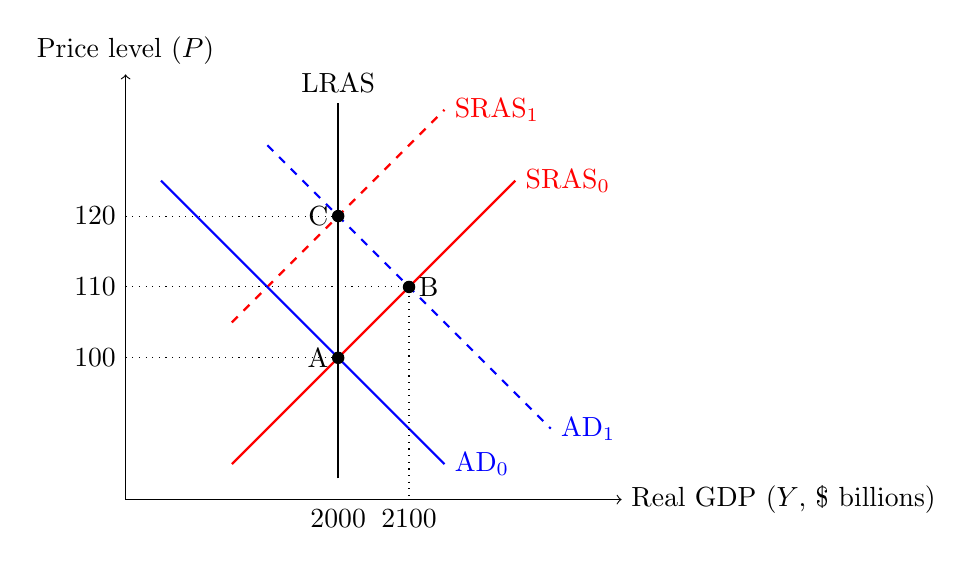
\begin{tikzpicture}[scale=0.9]
  \draw[->] (0,0) -- (7,0) node[right] {Real GDP ($Y$, \$ billions)};
  \draw[->] (0,0) -- (0,6) node[above] {Price level ($P$)};
  \draw[thick] (3,0.3) -- (3,5.6) node[above] {LRAS};
  \draw[thick, red] (1.5,0.5) -- (5.5,4.5) node[right] {SRAS$_0$};
  \draw[thick, red, dashed] (1.5,2.5) -- (4.5,5.5) node[right] {SRAS$_1$};
  \draw[thick, blue] (0.5,4.5) -- (4.5,0.5) node[right] {AD$_0$};
  \draw[thick, blue, dashed] (2,5) -- (6,1) node[right] {AD$_1$};
  \fill (3,2) circle (2.5pt) node[left] {A};
  \fill (4,3) circle (2.5pt) node[right] {B};
  \fill (3,4) circle (2.5pt) node[left] {C};
  \draw[dotted] (0,2) node[left] {100} -- (3,2);
  \draw[dotted] (0,3) node[left] {110} -- (4,3) -- (4,0) node[below] {2100};
  \draw[dotted] (0,4) node[left] {120} -- (3,4);
  \node[below] at (3,0) {2000};
\end{tikzpicture}
\end{center}

\begin{example}[An increase in AD and the adjustment to long-run equilibrium]
Let potential GDP be \$2{,}000 billion, with
\[
  \text{AD}_0: Y = 3000 - 10P, \qquad \text{SRAS}_0: Y = 1000 + 10P.
\]
Short-run equilibrium: $3000 - 10P = 1000 + 10P \implies P = 100$, $Y = 2000$. Since
$Y$ equals potential GDP, this is also long-run equilibrium (point A).

Now an export boom shifts AD to $\text{AD}_1: Y = 3200 - 10P$. With money wages fixed:
\[
  3200 - 10P = 1000 + 10P \implies P = 110, \quad Y = 2100 \quad (\text{point B}).
\]
Real GDP exceeds potential by 100: an \emph{inflationary gap}. Unemployment is below the
natural rate, so money wages rise and SRAS shifts leftward. The process stops when real
GDP is back at 2000 on AD$_1$: $2000 = 3200 - 10P \implies P = 120$ (point C). The new
SRAS passes through $(2000, 120)$; with the same slope it is
$\text{SRAS}_1: Y = 800 + 10P$. In the long run, the increase in AD raised only the price
level (by 20\%).
\end{example}

\subsection{Output gaps}

\begin{itemize}
  \item \textbf{Inflationary gap}: real GDP $>$ potential GDP. Money wages rise, SRAS
        shifts left, the price level rises and real GDP falls back to potential.
  \item \textbf{Recessionary gap}: real GDP $<$ potential GDP. Unemployment exceeds the
        natural rate; money wages fall (slowly), SRAS shifts right, the price level falls
        and real GDP rises back to potential. Because money wages are sticky downward, this
        adjustment can take a long time, which is the case for stabilization policy.
\end{itemize}

\subsection{Economic growth, inflation and the business cycle}

\begin{itemize}
  \item \textbf{Economic growth}: potential GDP grows (more labour, capital, technology), so
        LRAS shifts rightward over time.
  \item \textbf{Inflation}: if AD grows faster than LRAS (mainly because the quantity of
        money grows faster than potential GDP), the price level rises persistently.
  \item \textbf{The business cycle}: AD and SRAS grow at uneven rates, so short-run
        equilibrium real GDP fluctuates around potential GDP, creating alternating
        inflationary and recessionary gaps.
\end{itemize}

\subsection{Fluctuations in aggregate demand}

A decrease in AD (e.g.\ the 2008--2009 collapse in world demand for Canadian exports) moves
the economy down along SRAS: real GDP and the price level both fall, creating a
recessionary gap. An increase in AD creates an inflationary gap as in the example above.

\begin{center}
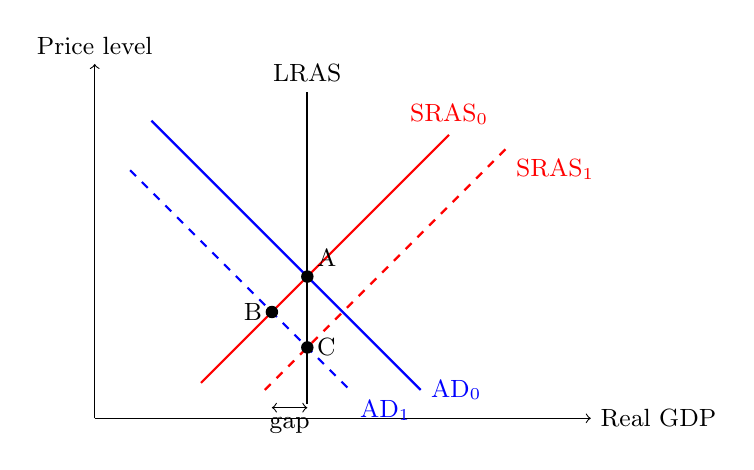
\begin{tikzpicture}[scale=0.9, every node/.style={font=\small}]
  \draw[->] (0,0) -- (7,0) node[right] {Real GDP};
  \draw[->] (0,0) -- (0,5) node[above] {Price level};
  \draw[thick] (3,0.2) -- (3,4.6) node[above] {LRAS};
  \draw[thick, red] (1.5,0.5) -- (5,4) node[above] {SRAS$_0$};
  \draw[thick, red, dashed] (2.4,0.4) -- (5.8,3.8) node[below right] {SRAS$_1$};
  \draw[thick, blue] (0.8,4.2) -- (4.6,0.4) node[right] {AD$_0$};
  \draw[thick, blue, dashed] (0.5,3.5) -- (3.6,0.4) node[below right] {AD$_1$};
  \fill (3,2) circle (2.5pt) node[above right] {A};
  \fill (2.5,1.5) circle (2.5pt) node[left] {B};
  \fill (3,1) circle (2.5pt) node[right] {C};
  \draw[<->] (2.5,0.15) -- node[below] {gap} (3,0.15);
\end{tikzpicture}
\end{center}
AD falls from AD$_0$ to AD$_1$: the economy moves from A to B, below potential GDP, with a
lower price level. Only as money wages slowly fall does SRAS shift right (SRAS$_1$), taking
the economy to C at potential GDP and an even lower price level.

\subsection{Fluctuations in aggregate supply}

A rise in the price of oil (or another key input) increases costs and shifts SRAS
leftward without changing potential GDP. Real GDP \emph{falls} and the price level
\emph{rises}: a combination called \emph{stagflation} (as in the 1970s). Policy faces a
dilemma: increasing AD to restore output raises the price level further; doing nothing
leaves a recessionary gap until money wages fall.

\begin{center}
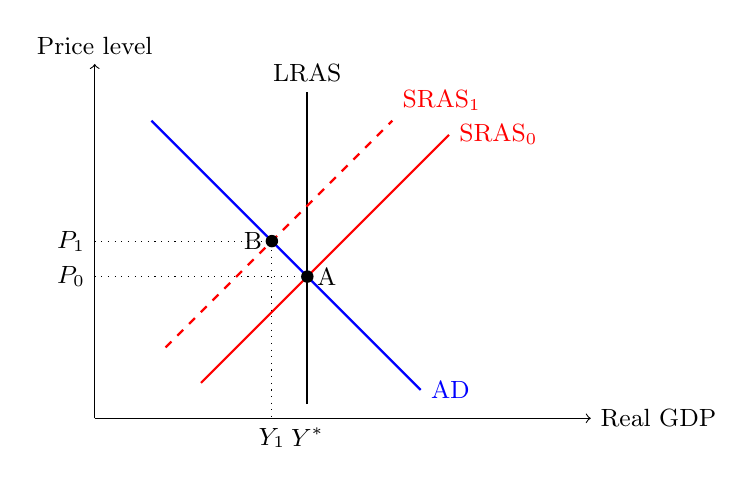
\begin{tikzpicture}[scale=0.9, every node/.style={font=\small}]
  \draw[->] (0,0) -- (7,0) node[right] {Real GDP};
  \draw[->] (0,0) -- (0,5) node[above] {Price level};
  \draw[thick] (3,0.2) -- (3,4.6) node[above] {LRAS};
  \draw[thick, red] (1.5,0.5) -- (5,4) node[right] {SRAS$_0$};
  \draw[thick, red, dashed] (1,1) -- (4.2,4.2) node[above right] {SRAS$_1$};
  \draw[thick, blue] (0.8,4.2) -- (4.6,0.4) node[right] {AD};
  \fill (3,2) circle (2.5pt) node[right] {A};
  \fill (2.5,2.5) circle (2.5pt) node[left] {B};
  \draw[dotted] (0,2) node[left] {$P_0$} -- (3,2);
  \draw[dotted] (0,2.5) node[left] {$P_1$} -- (2.5,2.5) -- (2.5,0) node[below] {$Y_1$};
  \node[below] at (3,0) {$Y^{*}$};
\end{tikzpicture}
\end{center}
A cost shock moves the economy from A to B: real GDP falls below potential while the
price level rises.

\begin{important}[Summary of shifts]
\begin{center}
\begin{tabular}{lcc}
\toprule
Shock & Short run: $Y$ & Short run: $P$ \\
\midrule
AD increases & up & up \\
AD decreases & down & down \\
SRAS decreases (cost rise) & down & up \\
SRAS increases & up & down \\
LRAS and SRAS increase (growth) & up & down (or rises less) \\
\bottomrule
\end{tabular}
\end{center}
In the long run, AD changes affect only $P$; real GDP returns to potential.
\end{important}

\section{Macroeconomic schools of thought}

Macroeconomists broadly fall into three schools.
\begin{enumerate}
  \item \textbf{Classical.} The economy is self-regulating and always at full employment.
        The \emph{new classical} view is that business cycle fluctuations are the efficient
        responses of a well-functioning market economy bombarded by shocks that arise from
        the uneven pace of technological change. Policy should not try to smooth the
        cycle; taxes that blunt incentives are the main concern.
  \item \textbf{Keynesian.} Left alone, the economy would rarely operate at full
        employment; achieving and maintaining full employment requires active help from
        fiscal policy and monetary policy. The traditional view emphasizes sticky money
        wages and swings in ``animal spirits'' (expectations); the \emph{new Keynesian}
        view holds that not only money wages but also the prices of goods are sticky.
  \item \textbf{Monetarist.} The economy is self-regulating and will normally operate at
        full employment, provided monetary policy is not erratic and the pace of money
        growth is kept steady. Fluctuations come mainly from changes in the quantity of
        money (or interest rates).
\end{enumerate}
The AS--AD model is a framework that all three schools use; they disagree about how
quickly money wages adjust and which shocks matter most.

\section{Summary}

\begin{itemize}
  \item LRAS is vertical at potential GDP; SRAS slopes upward because money wages are
        fixed in the short run.
  \item Changes in potential GDP shift both LRAS and SRAS; changes in money wages or
        other resource prices shift only SRAS.
  \item AD slopes downward because of the wealth effect and the intertemporal and
        international substitution effects; it shifts with expectations, fiscal and
        monetary policy, the exchange rate and foreign income.
  \item Short-run equilibrium: AD $=$ SRAS. Long-run equilibrium: also on LRAS. Money wage
        adjustment closes inflationary and recessionary gaps.
  \item AD shocks move $Y$ and $P$ in the same direction; SRAS shocks move them in opposite
        directions (stagflation).
  \item Classical, Keynesian and monetarist views differ on self-regulation and the role
        of policy.
\end{itemize}
